\documentclass[UTF8]{ctexart}
\usepackage[paper=a4paper,dvips,top=2.5cm,left=2.8cm,right=2.8cm,foot=1cm,bottom=3.2cm]{geometry}
\usepackage{fancyhdr}
\usepackage{indentfirst}
\usepackage{enumerate}
\usepackage{clrscode}
\usepackage{listings}
\usepackage{amsmath}
\usepackage{amstext}
\lstset{language=Matlab}%代码语言使用的是matlab
\lstset{breaklines}%自动将长的代码行换行排版
\lstset{extendedchars=false}%解决代码跨页时,章节标题,页眉等汉字不显示的问题
\usepackage{graphicx}
\DeclareGraphicsExtensions{.eps,.ps,.jpg,.bmp}
\pagestyle{plain}
\author{王超民}
\title{消息链中的特定用户潜在影响力及敏感度学习}
\begin{document}
\maketitle
\par 本文研究的问题是从消息链中推测用户的影响力和敏感度,提出了一个数学模型LIS(Latent Influence and Susceptibility)。相较于之前的数学模型,LIS解决了严重的过拟合问题和充分利用了信息传播的上下文信息。
\par 过拟合问题源于在以往的模型中的一个假设:不同用户对之间的人际影响是独立无关的。LIS模型则针对特定用户行为,对用户之间的影响力建模。具体的,用两个$d$维的向量:影响力向量$I_{u}$和敏感度向量$S_{u}$,来表示用户$u$在$d$个潜在话题的影响力和敏感度。用户对$(u,v)$之间的人际影响可以通过计算$I_{u}$和$S_{u}$的内积得到。这种简明的表示方法对于$n$个用户而言,只需要$2nd(\ll n_{2})$个参数。
\section*{模型描述}
\par 给定一条消息$m$,记它的转发链$C^{m}$为按转发时间先后顺便排列的用户列表$(a_{1}^{m},\dots,a_{N}^{m})$。如果用户发布或者转发了这条消息,那么我们称用户是活跃的,并且他有一次机会去“激活”其他用户。至于“激活成功与否”,取决于当前时刻的上下文链。
\par \noindent \textbf{上下文链:}当活跃用户$a_{i}^{m}(i=1,\dots,N)$试图去“激活”某用户$v$时,此时的上下文链为
\begin{equation}
D_{v,i}^{m}=\left \{ a_{j}^{m} \mid j\leq i,\delta (a_{j}^{m},v)=1  \right \},
\end{equation}
其中指示器函数$\delta (u,v)$表示来自$u$的消息是否可以传递至$v$,我们将用过去所有的转发链和社会影响网络的叠加网络来表示,如图1所示。总之,上下文链代表着用户$v$此前接收到这条消息的那些用户列表。
\begin{figure}[h!]
    \centering
    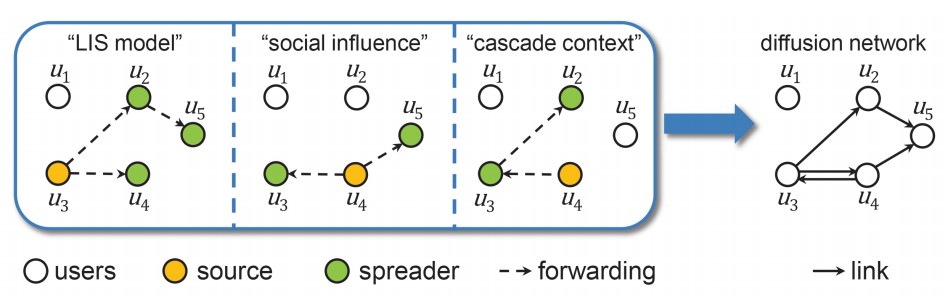
\includegraphics[width=12cm]{Fig1.jpg}
    \caption{图1 转发链的叠加}
    \label{fig-sample}
\end{figure}
\par 对于消息$m$及它的转发链$(a_{1}^{m},\dots,a_{N}^{m})$,每个用户可以用一个$N$维的状态向量$z_{v}^{m}$来表示,该状态向量的元素$z_{v,j}^{m}$代表用户$v$是否在接收到来自用户$a_{j}^{m}$的消息$m$后处于活跃状态。如果用户$v$从用户$a_{j}^{m}$的消息$m$后处于活跃状态,那么$z_{v,i}^{m}=0\;\;  (1\leq i< j)$,$z_{v,i}^{m}=1\;\;  (j\leq i< N)$。如果$v$在整个$m$的转发链都处于非活跃状态,那么对于任意的$i$,$z_{v,i}^{m}=0$。
\par $z_{v}^{m}$的似然函数为
\begin{equation}
P(z_{v}^{m}\mid \delta )=p(z_{v,0}^{m})\prod _{i=1}^{N}p(z_{v,i}^{m} \mid z_{v,i-1}^{m},D_{v,i}^{m} ,\delta)
\end{equation}
其中$z_{v,0}^{m}$表示$v$是否为消息$m$的始发者
\begin{equation}
p(z_{v,0}^{m}=1)= \left\{\begin{matrix}
\begin{aligned}
& 1,v\text{ is the source}&\\ 
& 0,\text{ otherwise} &
\end{aligned}
\end{matrix}\right.
\end{equation}
\begin{equation}
\begin{matrix}
\begin{aligned}
& p(z_{v,i}^{m}=1 \mid z_{v,i-1}^{m}=1,D_{v,i}^{m},\delta)=1 & \\
& p(z_{v,i}^{m}=1 \mid z_{v,i-1}^{m}=0,D_{v,i}^{m},\delta)=1-exp(-\lambda \delta(a_{v}^{m},v)\sum _{u \in D_{v,i}^{m}}I_{u}^{T}S_{v}) &\\
& p(z_{v,i}^{m}=0 \mid z_{v,i-1}^{m}=0,D_{v,i}^{m},\delta)=1-p(z_{v,i}^{m}=1 \mid z_{v,i-1}^{m}=0,D_{v,i}^{m},\delta) &
\end{aligned}
\end{matrix}
\end{equation}
其中$\lambda$是比例因子,用来调整上下文链的影响。公式($4$)说明了转移概率是如何受到上下文链的影响。
\par 假设转发链不相关,则所有转发链$C$的似然函数为公式($2$)的乘积
\begin{equation}
L(C) = \prod _{m=1}^{\left | C \right |}\prod _{v \in V}P(z_{v}^{m} \mid \delta)
\end{equation}
\par LIS模型的参数通过最小化对数似然代价函数得到
\begin{equation}
\L (C) = -\sum _{m=1}^{\left | C \right |}\sum _{v \in V}\sum _{i=1}^{N}log\; p(z_{v,i}^{m}\mid z_{v,i-1}^{m}, D_{v,i}^{m},\delta)
\end{equation}
其中$p(z_{v,0}^{m})$总是为1。
\section*{参数估计}
\par 一般来说,可以直接最小化公式($6$)来完成参数$I$和$S$的估计。但是带来的过高计算量我们无法承受。同时,一条上下文链会在转发链中重复出现很多次,导致公式($4$)的大量重复计算。因此,我们将充分利用在多条转发链中的重叠上下文链来减少重复计算。
\par 记$\Gamma (v)$为关于v在所有转发链中的所有可能的上下文链。对上下文链进行用户分组,重组公式($6$)的对数似然函数为
\begin{equation}
\L (C) = -\sum _{v \in V}\sum _{D_{v,i}\in \Gamma (v)}^{N}(n_{z_{v,i},D_{v,i}}log \; p(z_{v,i}\mid z_{v,i-1}, D_{v,i},\delta)) 
\end{equation}
其中$D_{v,i}$表示用户$v$的一条与特定转发链无关的上下文链,$n_{z_{v,i},D_{v,i}}$为用户$v$在状态$z_{v,i}$下,$D_{v,i}$出现在所有转发链的频率。
\par 为了避免过拟合,我们需要对公式($7$)增加关于参数向量$I$和$S$的正则项,得到最终的参数估计目标函数
\begin{equation}
\begin{matrix}
\begin{aligned} 
& \L (C) = -\sum _{v \in V}\sum _{D_{v,i}\in \Gamma (v)}^{N}(n_{z_{v,i},D_{v,i}}log \; p(z_{v,i}\mid z_{v,i-1}, D_{v,i},\delta)) + \gamma _{I}\left \| I \right \|_{F}^{2}+\gamma _{S}\left \| S \right \|_{F}^{2} &\\ 
& s.t.\; I_{ij}\geq 0,S_{ij}\geq 0,\forall i,j &
\end{aligned}
\end{matrix}
\end{equation}
其中$\gamma _{I}$和$\gamma _{S}$为正则系数,$\left \| \cdot  \right \|_{F}$为Frobenius范数。
\par 最后,利用PG(Projected Gradient)法,我们设计了一种迭代算法完成参数估计。关于$I$和$S$的梯度
\begin{equation}
\begin{matrix}
\begin{aligned}
& \frac{\partial \L}{I_{u}}=-\lambda \sum _{v \in V}S_{v}\sum _{D_{v,i}\in \Gamma (v)} \Phi _{u \in D_{v,i}}(n_{z_{v,i}=1,D_{v,i}}\frac{1-p_{v,D_{v,i}}}{p_{v,D_{v,i}}}-n_{z_{v,i}=0,D_{v,i}})+\gamma _{I}I_{u} & \\
& \frac{\partial \L}{S_{v}}=-\lambda \sum _{D_{v,i}\in \Gamma (v)}\sum _{u \in D_{v,i}} I _{u}(n_{z_{v,u}=1,D_{v,u}}\frac{1-p_{v,D_{v,u}}}{p_{v,D_{v,u}}}-n_{z_{v,u}=0,D_{v,u}})+\gamma _{S}S_{v} & \\
\end{aligned}
\end{matrix}
\end{equation} 
其中$\Phi$为指示函数,$p_{v,D_{v,i}}$是$p(z_{v,i}=1\mid z_{v,i-1}, D_{v,i},\delta)$的简写。参数估计的算法见Algorithm 1。
\begin{codebox}[\indent ]
\Procname {Algorithm 1 参数估计}
\zi \kw{Input:} Collection of cascades observed in a given time period, the maximum epoch $M$, 
\zi and regularization parameters $\gamma_{I}$ and $\gamma_{S}$
\zi \kw{Output:} User-specific influence and susceptibility $I,S$
\zi
\zi Construct diffusion network $\delta$ from cascades
\zi Initialize parameters with random values, including $I,S$
\zi \Indentmore \kw{Repeat}
\zi \Indentmore \kw{For} $i=1$ to $n$ 
\zi   Calculate gradients $\partial L/ \partial I_{u}$ and $\partial L/ \partial S_{v}$
    \End 
\zi Update $I$ and $S$ with PG method
    \End 
\zi \kw{Until} maximum epoch $M$ is reached or gradients vanish
\end{codebox}

\end{document}
